% IEEE PAPER FORMAT 
\documentclass[twocolumn,oneside,conference]
{IEEEtran}

%%%%%%% all the required packages are loaded%%%%
\usepackage{filecontents}
\usepackage[style=ieee,backend=biber]{biblatex}
\usepackage{graphicx}
\usepackage{lmodern}	
\usepackage{enumerate}
\usepackage{float}


% bibilography page%%%%%%%%%%%%%%
\begin{filecontents}{Master.bib}


@article{5,
author = {Fill later},
title = {APP locus duplication causes autosomal dominant early-onset Alzheimer disease with cerebral amyloid angiopathy},
journaltitle = {Nat Genet.},
year = {2006},
volume = {38},
number = {1},
month = {Jan},
pages = {24-26},
doi = {10.1038/ng1718},
}


@article{first,
author = {Redon~et~al.},
title = {Global variation in copy number in the human genome},
journaltitle = {Nature},
year = {2006},
doi = {10.1038/nature05329},
}
@article{2,
author = {Alkan~et~al.},
title = {Genome structural variation discovery and genotyping},
journaltitle = {Nat Rev Genet},
year = {2011},
volume = {12},
number = {5},
month = {May},
pages = {363-376},
doi = {10.1038/nrg2958},
}

@article{3,
author = {Sebat~J~et~al.},
title = {Strong association of de novo copy number mutations with autism},
journaltitle = {Science},
year = {2007},
month = {Mar},
pages = {445-449},
volume = {361},
number = {5823},
doi = {10.1126/science.1138659},
}

@article{4,
author = {Hreinn Stefansson~et~al.},
title = {Large recurrent microdeletions associated with schizophrenia},
journaltitle = {Nature},
year = {2008},
volume = {455},
number = {7210},
month = {September},
pages = {232-236},
doi = {10.1038/nature07229},
}



\end{filecontents}
%%%%%%%%%%%%%%%%%%%%%%%%%%%%%%%%%%%%%%%



\addbibresource{Master.bib}

\IEEEoverridecommandlockouts 
\renewcommand\IEEEkeywordsname{Keywords}
\renewcommand*\finentrypunct{.}


\title{ICNV-TV: A read-depth based Copy Number Variation detection tool}
\markboth{Journal of Not yet Decided}{Sriharsha \MakeLowercase{\textit{et al}}: A read-depth based Copy Number Variation detection tool}

\author{
	\IEEEauthorblockN{Sriharsha Vogeti} 
	\IEEEauthorblockA{CCNSB,IIIT-Hyderabad\\
	vogetisri.harsha@research.iiit.ac.in}
	\and
	\IEEEauthorblockN{Prashanthi D} 
	\IEEEauthorblockA{CCNSB,IIIT-Hyderabad\\
	prashanthi.d@research.iiit.ac.in}
	\and
	\IEEEauthorblockN{Nita Parekh} 
	\IEEEauthorblockA{CCNSB, IIIT-Hyderabad\\
	nita@iiit.ac.in}
	
}

\begin{document}
\maketitle


 
\begin{abstract}
Copy Number Variation (CNV) is a form of structural variation contributing significantly to variations found in human genomes. A number of studies, so far have shown that CNVs are associated with complex diseases. Micro-array genomic comparative hybridization   (arrayCGH)and fluorescence in situ hybridization (FISH) provided were limited by the low resolution offered. The advancement in sequencing technologies leading to the development of Next Generation Sequencing (NGS) techniques solved this problem by offering very high resolution. We develop a read-depth (RD) based pipeline called ICNVTV, having a total variation penalized least squares model for segmentation which was proposed by Duan et al 2013. A comprehensive testing, followed by comparison against other RD-based tools was done on simulated data and real data. We analysed results obtained from applying our method to five different populations belonging to South Asian region. Both the real data and population data were obtained from 1000Genome Project. \\
\end{abstract}
 
\begin{IEEEkeywords}
CNV Detection, CNVTV, Read-Depth Methods, Population Studies, NGS\\
\end{IEEEkeywords}
\section{Introduction}
\IEEEPARstart{C}opy Number Variation (CNV) is a form of structural variation (SV) defined as a DNA segment that is 1kb or larger and is present at a variable copy number when compared to the reference genome \cite{first}. Alkan et al \cite{2} puts a much lower threshold on the size of a SV to be called as CNV at 50bp. It is estimated that about 12\% of human genome across populations is subject to copy number variation \cite{first}. CNVs have made important contributions to human evolution, diversity \cite{7} and diseases.Several studies have shown the association of CNVs with complex diseases such as autism \cite{3}, schizophrenia \cite{4}, Alzheimer disease \cite{5}, cancer \cite{6}, etc. Initially for the detection of CNVs was carried out using FISH \cite{9}, comparative arrayCGH and SNP mircoarrays \cite{10}. The main disadvantages with these techniques were hybridization noise, limited coverage for genome and low resolution.The resolution offered by this techniques was around 10-25 kbp when 1 million probes where used \cite{8}. The development of Next generation Sequencing techniques has solved this problem. The main advantages of NGS techniques for sequencing are high throughput, low cost, high coverage and resolution \cite{11}. 

\par There are five methodologies to detect CNVs from NGS data \cite{11}. They are a) Read Depth (RD) or Depth of Coverage (DOC) b) split read c) paired-end method (PEM) d) denovo of assembly of genome and e) combinatorial approach. Depth of coverage is the most widely used method for CNV detection.DOC assumes that the copy of a region in a genome is proportional to the read depth at that position.We developed a DOC based CNV detection method for whole genome data, which uses total variation penalized least square model by Duan et al. 2013 \cite{12} for segmentation process. This method by Duan et al has been showed to detect CNVs of smaller sizes. 
\par We validate our method on simulated data and real data from 1000 Genomes Project \cite{16} and compare its  performance with three other DOC method based tools viz., ReadDepth \cite{13}, CNVnator \cite{14} and ControlFREEC \cite{15} in terms of sensitivity and specificity. We demonstrate our method's high specificity with a relatively good sensitivity on simulated data. Our method is also successfully able to distinguish between homozygous deletion and gaps in the reference genome, which other methods under consideration fail to do. We then apply our method to five populations viz.,\textit{ Bengali from Bangladesh} (BEB), \textit{Gujarati Indian from Houston} (GIH), \textit{Punjabi from Lahore} (PJL), \textit{Sri Lankan Tamil from the UK} (STU) and \textit{Indian Telugu from the UK} (ITU) belonging to South Asian super-population also from 1000 Genomes Project. We compare and contrast the results obtained in detail. 

\section{Methods}
\subsection{The Proposed Approach}
In this section we describe about our method in detail. A general CNV detection method can be data preprocessing, segmentation and post-processing. Below we brief about each stage and our approach at each stage.
\subsubsection{Data Preprocessing}
Most of the tools use alignment file (BAM/SAM) as the input. The read depth (RD) values can be calculated from the alignment files. These RD values calculated are not necessarily proportional to the underlying copy number. This is because of biases such as GC-content bias and mappability bias and random variations. Such RD values obtained can give raise to false positive calls. Hence, it is necessary to remove such effects to obtain true RD values. 

\paragraph*{GC-bias Correction}
GC-bias is the dependence between read depth and GC-content of region. GC-bias leads to under-representation of DNA fragments with high GC or high AT content. We use an algorithm given by Benjamani and Speed \cite{17}. They show that the GC-bias at a particular region is determined the GC composition of the full fragment to which it belongs. They use GC composition of the full fragment and then use it to correct the RD value at that position.

\paragraph*{Mappability and Read Quality}
Mappability for a region in the reference genome is defined
as the probability that a read originating from it is unambiguously mapped back to it. Regions with repetitive elements have a low mappability. Reads generating from such regions are ambiguously mapped and have a low mappability score, leading to higher RD values. We ignore regions/bins with a mappability score (which lies between 0 and 1 including) of 0.5 for CNV detection. We also filter reads with a mapping quality score of zero (q0 reads). We used samtools \cite{18} to filter out low quality reads.

\paragraph*{Binning}
Binning is the process in which RD values of a small intervals, called as bins are replaced by a value, generally average of RD values in that bin, as a representative of that bin. Binning is done to reduce the effects of random sequencing errors. Bin length (window length) is an optional parameter in our method, with a default value of 100bp. RD values were calculated using bedtools \cite{19}. We will describe in detail on how bin length affects the CNV detection in later sections.         


\subsubsection{Segmentation}
Segmentation can be described as the process of divided the regions into segments such that bins in a region will have similar RD values. A majority of the CNV detection methods use statistical models such as Circular Binary segmentation, Mean Shift algorithm, Hidden Morkhov Model, etc. Duan J et al., 2011 proposes a total variation penalized least squares model for segmentation \cite{20}. They prove that their algorithm works better when compared to many tools in detecting CNVs with smaller window/bin size \cite{12}. We implement their algorithm in our method. The main reason for choosing it was its ability to detect smaller CNVs, given that the smaller SVs (between 50bp and 1000bp) were also being treated as CNVs.  

\subsubsection{Postprocessing}
 This stage involves identifying regions with abnormal copy number and determining their absolute copy numbers. To do so determination of upper and lower thresholds is done. For generally thresholds as simple as 1.5X and 0.5X of the average RD value are used as upper and lower threshold respectively. We use a slightly less strength viz., 1.45X and 0.55X of the average RD value as upper and lower thresholds respectively.   

\section{Results}
Discussion about what has been done
\subsection{Simulated Data}
\subsection{Real Data Analysis}
\subsection{Sub-population Analysis}
\begin{figure*}[h]
	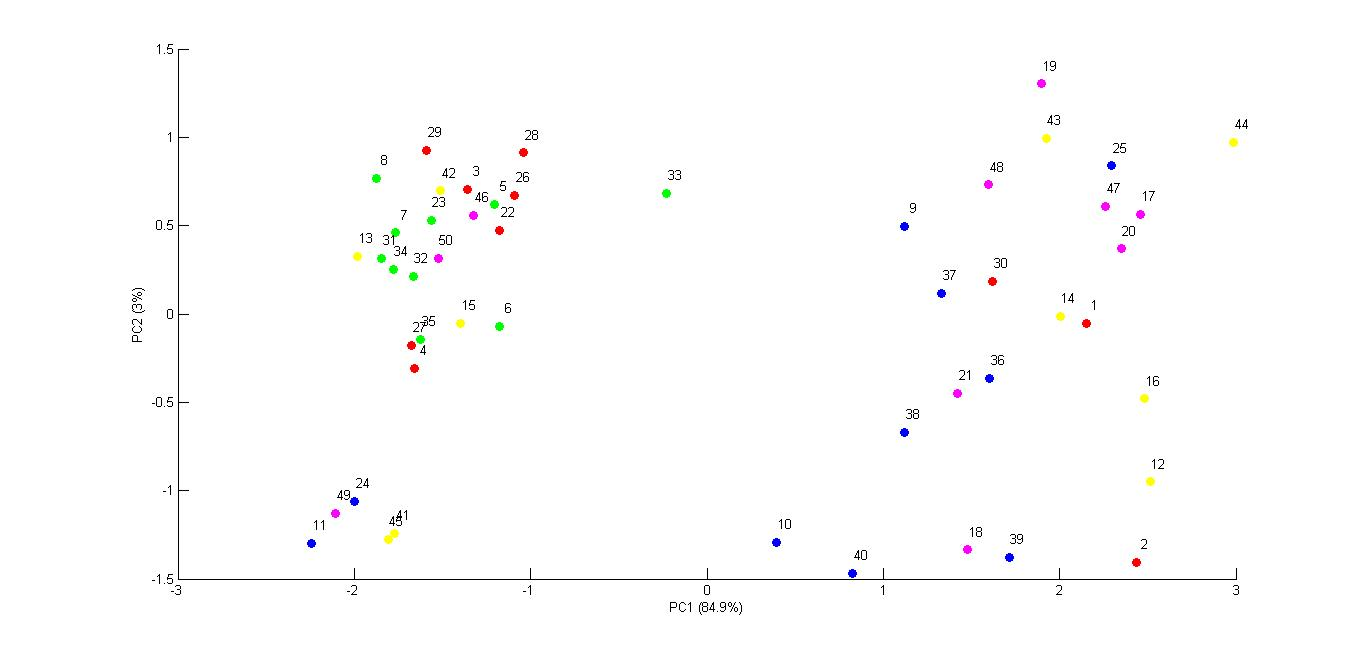
\includegraphics[width=\textwidth]{final.jpg}
	\caption{This is a test image}
	\label{fig1: this is test image}
\end{figure*}

\section{Discussion}

\section{Future work}

\section*{Acknowledgments}


\printbibliography

\end{document}



